\cotefile{134-2}
\scanpage{146}\mspage{1}
\hfill Villecun 17/19 \unsure{Juillet|juillet}\\
\hfill 1975\\
Cher Larry,\\

Tout d'abord félicitations pour la naissance de ta fille, qui heureusement ne s'est pas laissée impressionner par les importantes cogitations mathématiques de son papa -- au risque de les perturber quelque peu.

Au fait, quelle est ta situation en France : es\deleted{\unsure{t}}-tu français ou américain, prof. associé ou titulaire ? Si cela pouvait s'arranger, \unsure{serait|serais} tu intéressé par une position \unsure{:|à} Montpellier ? Cela te dit-il quelque chose de venir à l'occasion à Montpellier -- ou à Villecun -- pour discuter de tes favoris avec moi -- pour le moment il n'y a guère que moi ici pour ne pas nager entièrement (seulement partiellement) dans ce que tu fais.

J'ai été content de finir par recevoir un écho à ma longue \unsure{épitre|épître} -- et même un début d'approche constructive pour \deleted{\illegible{1}} une théorie du type que je prévois. La construction que tu proposes de la notion de $n$-catégorie pas stricte, et du foncteur nerf, a certes le mérite \inserted{d'exister et} d'être une \unsure{premièr|première} approche précise, mais par ailleurs prête \deleted{\unsure{évidemment}} \inserted{bien sûr}, le flanc à des critiques évidentes : d'être très technique, peu intuitive (alors \unsure{qu'au|où au} niveau des $1$-cat. et
% archive sheet number: 146
\scanpage{147}\mspage{2}
\unsure{\={m}|m\textsuperscript{e}} des $2$-cat. tout parait si clair -- ``il n'y a qu'à suivre le bout de son nez''\dots) et enfin l'absence d'une définition d'un foncteur allant des ens. (semi) simpliciaux vers les $n$-groupoïdes. Ce foncteur correspond à une intuition géométrique si claire qu'une théorie qui ne l'inclurait pas me semblerait canularesque. Peut-être en \inserted{essayant d'}écri\deleted{\unsure{vant}}\unsure{re} (Comme une sorte de liste de voeux de Noël !) de façon assez complète et explicite les \deleted{relations} notions \deleted{\unsure{qu'on}}\unsure{dont on} voudrait disposer et les relations (foncteurs, équivalences etc) qui doivent les lier, arriverait-on finalement à une sorte de description axiomatique assez poussée \deleted{\unsure{pour}}\unsure{qui}, soit \unsure{donne|donner} la clef d'une construction ad-hoc explicite, soit \inserted{qui permette} à la rigueur d'énoncer et démontrer un th. d'existence et d'unicité d'une théorie du type souhaité.

Par ailleurs, n'ayant pas compris l'idée de Segal dans ta dernière lettre (que j'ai généreusement envoyée à Illusie\dots), je ne vois pas comment tu définis les $n$-cat. de Picard -- mais peu importe. Pour ce qui est des $n$-cat. de Picard ``strictes'', tout ce que je leur demande, c'est qu'ils forment finalement une \inserted{$(n+1)$-}catégorie $(n+1)$-équivalente à celle des complexes de chaines de longueur $n$. D'accord ? Je te remercie
% archive sheet number: 147
\scanpage{148}\mspage{3}
d'avoir rectifié dans mon esprit une erreur \unsure{grossière}, \unsure{dû|dûe} à ma grande ignorance de la top. algébrique et de l'homotopie -- j'étais en effet dans le sentiment que les $H$-espaces satisfaisant des conditions d'associativité et commutativité assez strictes (disons équivalent à des ${\unsure{\Omega|{}'\!\Omega}}^{i}X$ avec $i$ arbitrairement grand) correspondaient à des groupes topologiques commutatifs (en m'inspirant de quelques analogies \dots). Donc entièrement d'accord avec tes observations p.~5.

Par contre, je suis toujours intrigué par la question suivante : n'y a-t\unsure{'|-}il pas un analogue du tapis de Dold-Puppe pour les groupes ($1/2$) simpliciaux (pas néc. commutatifs) et quelle forme prend-il ? À vrai dire, je considère le yoga
\diagram{\begin{tikzcd}[ampersand replacement=\&]
\text{ens. }1/2\text{ simplicial}\arrow[leftrightarrow,r] \& \infty\text{-}\deleted{\unsure{\text{catégorie}}}\text{groupoïde}
\end{tikzcd}}
comme étant essentiellement la version ``set-theoretic'' ultime de Dold-Puppe, qui s'en déduirait en explicitant seulement que les groupes abéliens dans $(\infty\text{-cat})$ ne ``sont autres'' que les complexes de chaines dans $(\mathrm{Ab})$. Il faudrait donc déterminer quels sont les groupes de $(\infty\text{-cat})$ : Je peux te dire ce qu'il en est dans $(1\text{-cat})$ -- ce sera dévelop%
% archive sheet number: 148
\scanpage{149}\mspage{4}%
pé en long et en large dans le livre de Mme Sinh, je pense, sous le titre de chapitre des ``Gr-catégories \uline{strictes}'' (i.e. \inserted{\unsure{où}} les isomorphismes d'associativité, d'unité, et d'inverse $X\mathbin{.}X^{-1}\unsure{\simeq|=}1$ sont des \uline{identités}). On peut expliciter p.ex. comment (via le fait que \unsure{tte|toute} Gr-cat. est Gr-équivalente à une Gr-catégorie stricte) le calcul avec les Gr-catégories se \unsure{réduit} à un calcul très algébrique avec des Gr-catégories \uline{strictes}, par une sorte de ``calcul des fractions'' (à droite ou à gauche, au choix) du type de celui qui \unsure{aboutit} à la construction des catégories dérivées. Quoi qu'il en soit, voici l'explicitation de cette structure (groupe dans $(1\text{-ct.})$) en termes de théorie des groupes ($1$-catégorie dans $(\mathrm{Gr})$) :

La structure est décrite par un quadruplet $(L_1,L_0,d,\unsure{\Theta|\theta})$, avec
\diagram{\begin{tikzcd}[ampersand replacement=\&]
L_1 \arrow[r,"d"] \& L_0
\end{tikzcd}}
un hom de groupes ordinaires, et
\[
\Theta:L_0\longrightarrow\underline{\mathrm{Aut}}_{\mathrm{gr}}(L_1)
\]
une opération de $L_0\deleted{\unsure{\Theta|0}}$ sur $L_1$, avec les
% archive sheet number: 149
\scanpage{150}\mspage{5}
deux axiomes suivants

a) $d$ commute aux op. de $L_0$, quand on le fait opérer sur $L_1$ par $\unsure{\Theta|\theta}\deleted{\unsure{,|s}}$, sur lui-même par aut. int :
\[
d\bigl(\Theta(x_0)\mathbin{.}x_1\bigr)=\mathrm{int}(x_0)\,d(x_1)
\]
\[
\Theta(d.(x_1))=\mathrm{int}(x_1)\tag*{\makebox[0pt][r]{\makebox[\displaywidth][l]{b)}}}
\]
Ces propriétés impliquent que $\mathrm{Im}\,d$ est \unsure{invariant} dans $L_0$ (donc $\unsure{\mathrm{Coker}|\mathrm{CoKer}}\,d=\unsure{\pi|\Pi}_0$ est défini) et $\pi_1=\mathrm{Ker}\,d$ est central dans $L_1$, enfin que $L_0$ opère sur $L_1$ en invariant $\pi_1$, et qu'il opère via $\pi_0$. Le principal invariant \inserted{coh.} de la situation est évidemment l'inv. de \unsure{Postnikoff|Postnikuff}-Sinh
\[
\alpha\in\unsure{.}\,H^3(\pi_0,\pi_1).
\]

J'ai rencontré ces animaux -- sans même les chercher -- dans pas mal de situations, que je ne vais pas te passer en revue ici (je viens d'ailleurs de \unsure{retomber} encore dessus à propos de la classification des groupes formels ``ordinaires'' \unsure{sur} un corps parfait, en termes de groupes algébriques \uline{affines}, de groupes formels \uline{commutatifs}, reliés par des Gr-structures strictes de ce type%
% margin note written sideways
\inserted{\illegible{4} ce formalisme sur un topos quelconque (pas seulement dans $(\mathrm{Ens})$)} -- pour expliciter le yoga que ``le caractère transcendant du
% archive sheet number: 150
\scanpage{151}\mspage{6}
groupe formel est concentré en les groupes formels commutatifs, découvert semble-t-il par Dieudonné \dots). La question que je voudrais soulever est la généralisation aux groupes dans $(n\text{-cat})$, on s'attend à trouver des complexes de chaines non \unsure{comm|comm.}
\diagram{\begin{tikzcd}[ampersand replacement=\&,column sep=small]
L_n\arrow[r,phantom,"\unsure{\text{---}|\longrightarrow}" description] \& L_{n-\unsure{1|,}}\arrow[r,no head,to path={-- (\tikztotarget) -- ++(0.025,0.055)}] \& \ldots\arrow[r,no head,to path={-- (\tikztotarget) -- ++(0.025,0.055)}] \& L_1\arrow[r,no head,to path={-- (\tikztotarget) -- ++(0.025,0.055)}] \& L_0\arrow[r] \& 1
\end{tikzcd}}
avec des structures supplémentaires sans doute du type $\unsure{\Theta|\theta}$, mais lesquelles ? Il est entendu que la signification topologique de ces structures, c'est qu'elles expriment exactement les ``types d'homotopie tronqués en dim $\leq n$'' des groupes topologiques. \inserted{\unsure{ou encore} les types d'hom tronqués en dim $\leq n+1$ des espaces top ponctués connexes \dots)} As-tu des \unsure{candïdats|candidats} à proposer ?

\figure{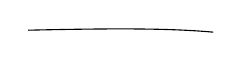
\begin{tikzpicture}\draw (0,0) .. controls (1.1,0.025) and (1.8,0.025) .. (2.35,-0.025);\end{tikzpicture}}

\unsure{.} Tes réflexions de bidualité \inserted{et d'homologie}, pour formelles qu'elles soient, se rattachent à une foule de développements, dont certains seulement existent\unsure{,} dès à présent, et d'autres demanderaient des développements considérables. Voici les réminiscences que m'\unsure{ouvrent|envoient} tes naïves questions :
% archive sheet number: 151
\scanpage{152}\mspage{7}%
A) Le formalisme des $Rf_!, f^!$ (combiné à $Rf_*, Lf^{\unsure{\alpha|*}}$, $\overset{\mathbb{L}}{\otimes}$ et $\mathbb{R}\mathrm{Hom}$, ``les six opérations'') porte implicitement en son sein la définition de l'homologie et l'identité essentielle entre \unsure{fonctions} homologiques et cohomologiques. \deleted{\unsure{E}} On dispose pour le moment de ce formalisme pour les faisceaux quasi-cohérents sur les schémas -- séminaire Hartshorne -- pour les espaces top. et les faisceaux de coeff. arbitraires dessus -- Verdier, exposé Bourbaki -- et en coh. étale des schémas pour les coefficients ``discrets'' \inserted{(de torsion ou ``$l$-adiques'')} \uline{premiers aux \deleted{\unsure{la|le}} car. résiduelles} -- SGA 5 -- \inserted{enfin pour les faisc. coh. sur les espaces analytiques -- Verdier-Ruget --}\,; (Le formalisme reste à développer dans le contexte cristallin, et en car. $0$ dans le contexte des modules stratifiés \inserted{à singularités} à la Deligne, avec éventuellement -- sur le corps $\mathbb{C}$ -- des structures de Hodge à la clef, enfin dans le contexte des motifs ; je suis persuadé qu'il est présent un peu partout encore -- partout, peut-être, où il y a un formalisme de nature cohomologique.) Travaillant en coh. étale sur un schéma \inserted{\unsure{séparé}} de t.f. sur un corps $k$, disons, avec un anneau de coeff. $\Lambda$ de torsion premier à la \unsure{car.|car}\unsure{,}
% archive sheet number: 152
\scanpage{153}\mspage{8}%
le \inserted{complexe de} faisceaux $f^!(\Lambda_e)$ (où $f:X\unsure{\text{---}|\longrightarrow}\operatorname{Spec} k=e$) joue le rôle du \uline{complexe des chaines singulières sur} $X$ \uline{à coeff. dans} $\Lambda$, et $Rf_!(f^!{\unsure{\Lambda|\mathbb{\Lambda}}}_e)$ joue le rôle d'une \uline{homologie} $H_*(X/e)$, vis à vis bien sûr de coefficients sur $e$ qui soient des complexes de $\Lambda$-modules. Tu justifieras aisément cette assertion à l'aide des ``th. de dualité globale'', par un ou deux tours de passe-passe que je t'épargne ici.

\uline{Remarques} 1) Il n'y a pas à tronquer, ça marche en toutes dimensions

2) C'est (au moins du p\textsuperscript{t} de vue philosophique) lié au fait qu'on dispose pour les coefficients envisagés \inserted{(sous condition de ``constructibilité\unsure{'')|)}} d'un th. de ``bidualité''\deleted{\unsure{)}}, du moins sous réserve de résolution des singularités (mais Deligne m'a dit je crois qu'il sait le prouver sans ça) à valeurs dans un ``complexe dualisant'' $K_e$ \inserted{(sur $e$)} $\unsure{\text{--}|;|\text{--};}$ $K_X$ (sur $X$). Si p.ex. $\Lambda$ est ``\unsure{autodual}'' \inserted{(ou Gorenstein)} p.ex. $\Lambda=\mathbb{Z}/n\mathbb{Z}$, on peut prendre $K_e=\Lambda$, donc \inserted{le complexe dualisant} $K_X=f^!(K_e)$ n'est autre que le ``complexe des chaines singulières à \unsure{coeff.} \unsure{dans} $\unsure{\Lambda}$'' \illegible{1}
% archive sheet number: 153
